\chapter{Progettazione Logica}
Ci vorrà ancora un po' per i risultati, ma non manca tanto.\\
La seconda parte, il secondo compitino, prevede 
\begin{itemize}
    \item la progettazione logica
    \item il secondo esercizio
    \item il terzo esercizio
\end{itemize}
Secondo il prof. Napoletano, la progettazione logica è abbastanza equiparabile al Modello Relazionale.\\
Viene presentato uno schema ER generico con proprietà ben determinate, senza una specifica, di cui bisogna identificare determinate regole di ristrutturazione prima di tradurre il modello destrutturato in un elenco di tabelle.
\section{Progettazione Logica}
\begin{center}
    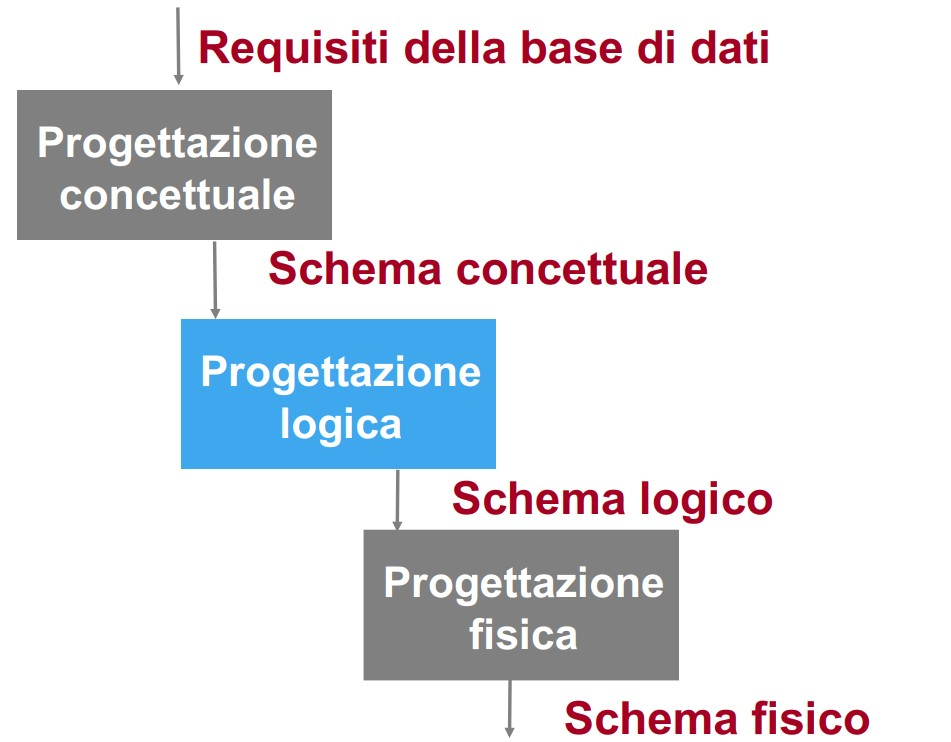
\includegraphics[scale=0.675]{chaptersLezioniSara/img/PLog_intro1.jpg}
\end{center}
Come già precedentemente detto, non vedremo a lezione la progettazione fisica (è prevista a laboratorio però).\\
Richiede di scegliere il modello dei dati modello relazionale.
\subsubsection{Obiettivo}
Definizione di uno schema logico relazionale corrispondente allo schema ER di partenza.
\subsubsection{Aspetti importanti}
Semplificazione dello schema per renderlo rappresentabile mediante il modello relazionale ottimizzazione per aumentare l'efficienza delle interrogazioni.

\subsection{Obiettivo}
"Tradurre" lo schema concettuale in uno schema logico che rappresenti gli stessi dati in maniera corretta ed efficiente.

\subsubsection{Ingresso:}
\begin{itemize}
    \item schema concettuale
    \item informazioni sul carico applicativo
    \item modello logico
\end{itemize}
\subsubsection{Uscita:}
\begin{itemize}
    \item schema logico
    \item documentazione associata
\end{itemize}
\begin{center}
    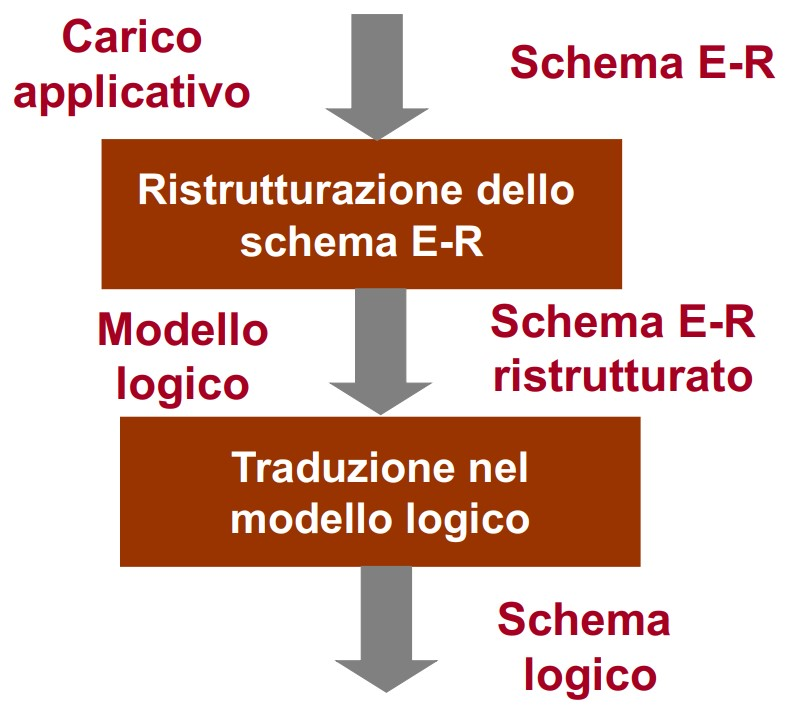
\includegraphics[scale=0.675]{chaptersLezioniSara/img/PLog_intro2.jpg}
\end{center}
Non si tratta di una pura e semplice traduzione
\begin{itemize}
    \item alcuni aspetti non sono direttamente rappresentabili
    \item è inoltre necessario considerare le prestazioni
\end{itemize}
\begin{center}
    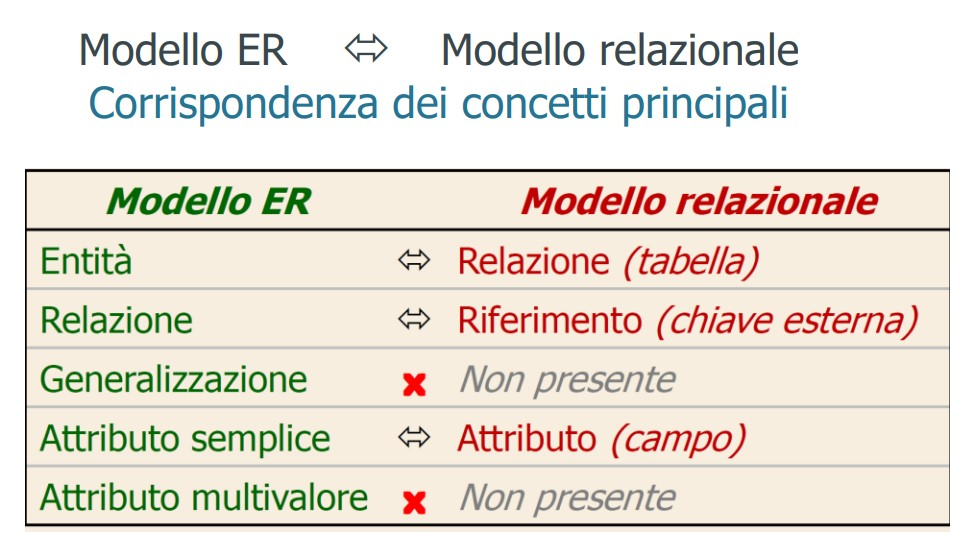
\includegraphics[scale=0.675]{chaptersLezioniSara/img/PLog_intro3.jpg}
\end{center}

\subsection{Ristrutturazione schema E-R}
Eliminazione dallo schema E/R di tutti i costrutti che non possono essere direttamente rappresentati nel modello logico target (relazionale nel nostro caso):
\begin{itemize}
    \item Eliminazione degli attributi multivalore
    \item Eliminazione delle generalizzazioni
\end{itemize}
Inoltre:
\begin{itemize}
    \item Partizionamento/accorpamento di entità e associazioni
    \item Scelta degli identificatori primari
    \item Analisi ridondanze (non dovrebbero esserci, \dots)
\end{itemize}
\begin{center}
    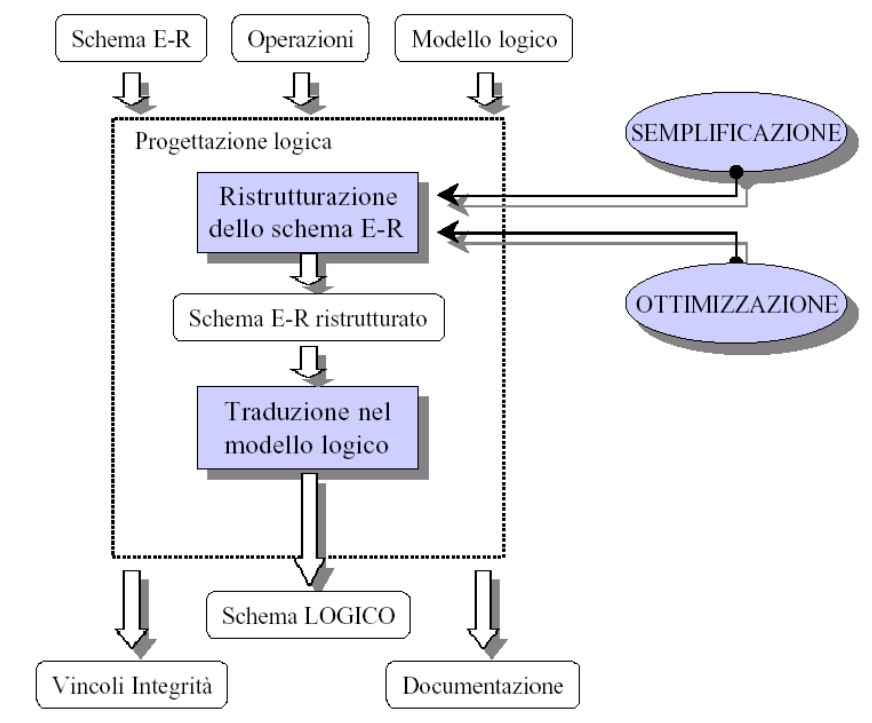
\includegraphics[scale=0.675]{chaptersLezioniSara/img/PLog_intro4.jpg}
\end{center}
\subsubsection{Motivazioni:}
\begin{itemize}
    \item semplificare la traduzione
    \item "ottimizzare" le prestazioni
\end{itemize}
\subsubsection{Osservazione:}
\begin{itemize}
    \item uno schema E-R ristrutturato non è (più) uno schema concettuale nel senso stretto del termine
\end{itemize}
\textbf{Per ottimizzare il risultato abbiamo bisogno di analizzare le prestazioni a questo livello.}\\
Ma:
\begin{itemize}
    \item le prestazioni non sono valutabili con precisione su uno schema concettuale:
    \item Dipendono dalle caratteristiche del DBMS
    \item bisogna conoscere il volume dei dati e le caratteristiche delle operazioni
\end{itemize}

\subsection{Carico applicativo}
Consideriamo degli "indicatori" dei parametri che regolano le prestazioni:
\begin{itemize}
    \item \textit{tempo di esecuzione} delle operazioni di principale interesse: numero di istanze (di entità e relazioni) mediamente accedute durante l'esecuzione dell'operazione \textit{(accessi)}
    \item \textit{spazio di memoria} necessario per memorizzare i dati di interesse
\end{itemize}
Per valutare questi parametri bisogna conoscere (oltre allo schema):
\subsubsection{volume dei dati:}
\begin{itemize}
    \item numero di istanze previste di entità e relazioni
    \item dimensione di ciascun attributo
\end{itemize}
\subsubsection{caratteristiche delle operazioni:}
\begin{itemize}
    \item tipo: interattiva o batch
    \item frequenza: numero medio di esecuzioni in un certo periodo
    \item dati coinvolti
\end{itemize}
Si noti che la valutazione sarà necessariamente approssimata, in quanto le prestazioni effettive della base di dati dipendono anche da parametri fisici, difficilmente prevedibili in questa fase (DBMS utilizzato, indici, \dots).

\subsection{Schema di operazione}
Lo schema di operazione descrive i dati coinvolti in un'operazione.\\
Corrisponde al frammento dello schema ER interessato all'operazione sul quale viene disegnato il cammino logico per accedere alle informazioni di interesse.\\
\begin{center}
    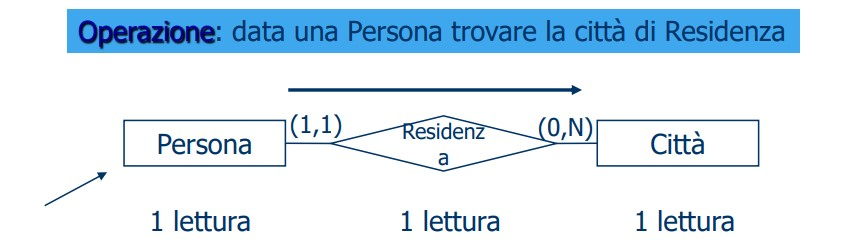
\includegraphics[scale=0.675]{chaptersLezioniSara/img/PLog_intro5.jpg}
\end{center}
Ma perché questo schema è importante? Per le operazioni che devo affrontare che possono essere molto ripetitive.

\subsection{Esempio 1}
\begin{center}
    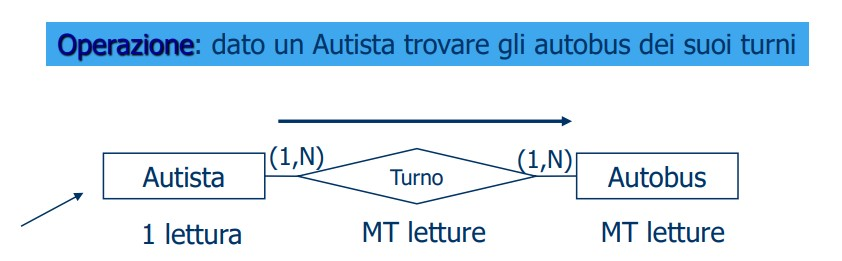
\includegraphics[scale=0.675]{chaptersLezioniSara/img/PLog_intro_es1.jpg}
\end{center}
Per calcolare il numero di accessi a Turno e Autobus occorre conoscere il numero medio di Turni per Autista (MT).

\subsection{Tavola degli accessi}
Con lo schema di operazione si può fare una stima del costo di un'operazione contando il numero di accessi alle istanze di entità e relazioni.\\
Il risultato può essere riassunto in una \textbf{tavola degli accessi}.
\begin{center}
    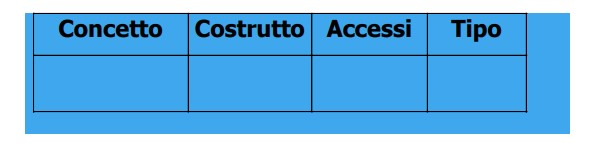
\includegraphics[scale=0.675]{chaptersLezioniSara/img/PLog_tavolaAccessi1.jpg}
\end{center}
Il tipo distingue gli accessi in scrittura (S) e in lettura (L).\\
Le operazioni di scrittura sono in genere più onerose (esecuzione in modo esclusivo, aggiornamento degli indici).

\subsection{Esempio 1}
\begin{center}
    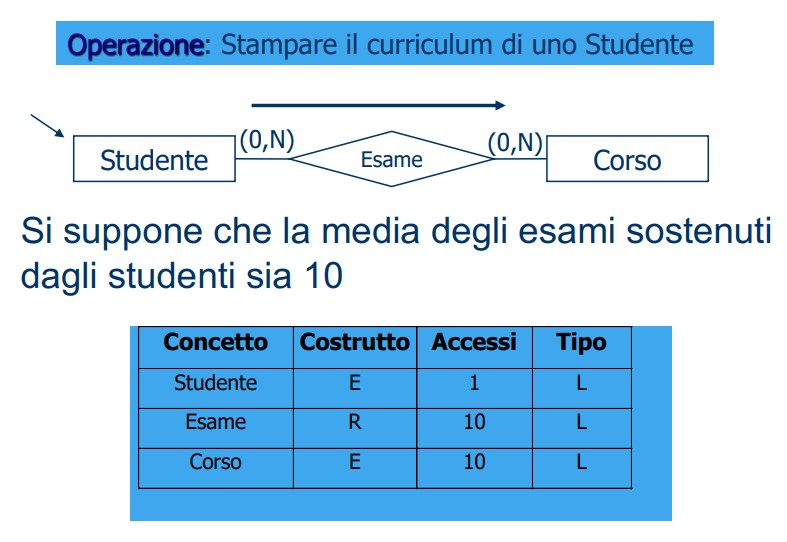
\includegraphics[scale=0.675]{chaptersLezioniSara/img/PLog_tavolaAccessi_es1.jpg}
\end{center}
\subsection{Esempio 2}
\begin{center}
    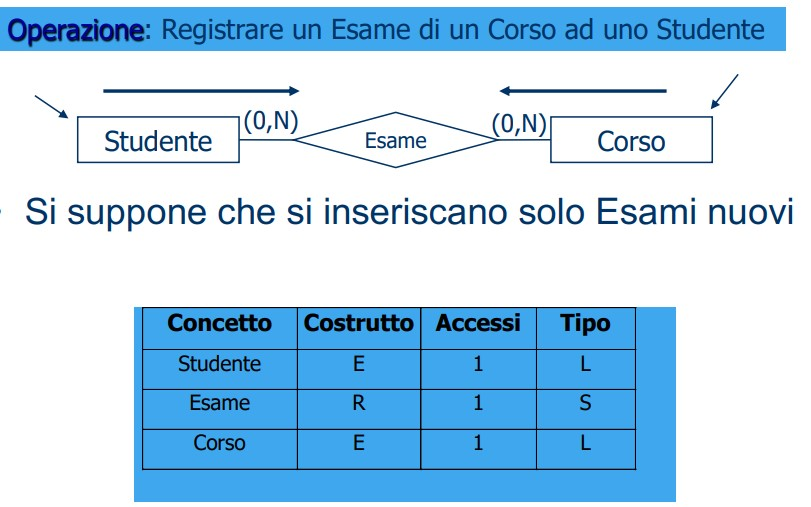
\includegraphics[scale=0.675]{chaptersLezioniSara/img/PLog_tavolaAccessi_es2.jpg}
\end{center}

\subsection{Esempio di valutazione di costo}
Schema E-R:
\begin{center}
    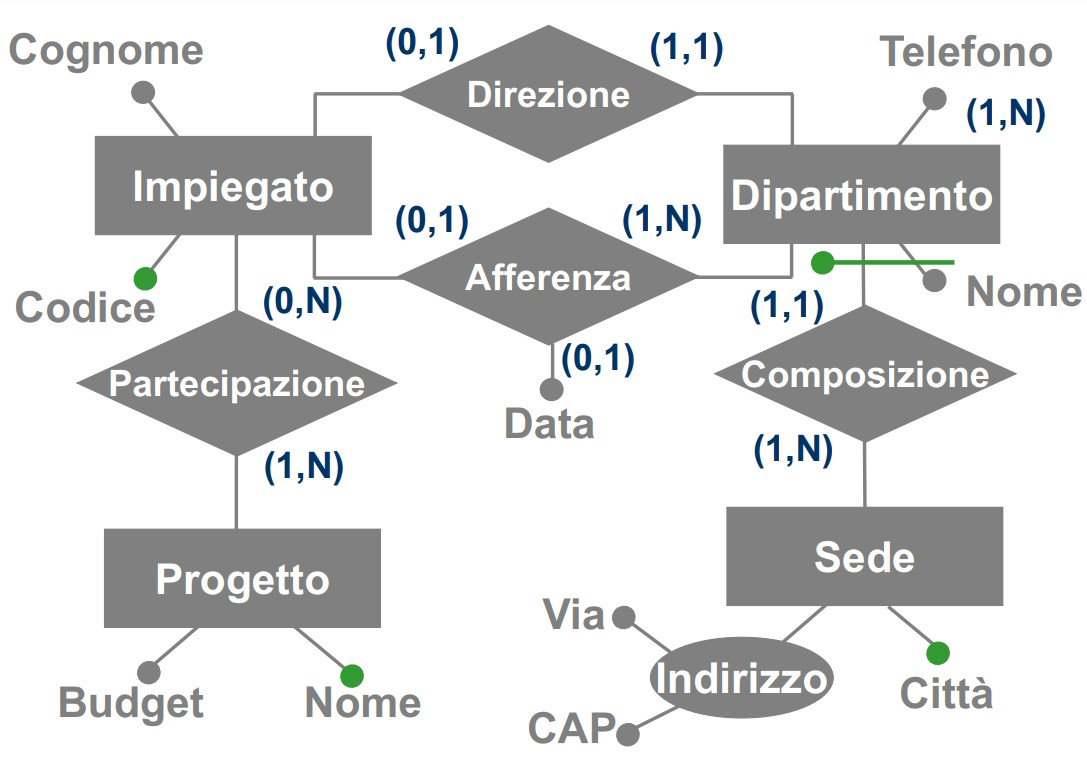
\includegraphics[scale=0.675]{chaptersLezioniSara/img/PLog_tavolaAccessi_es3a.jpg}
\end{center}
\begin{description}
    \item[Operazione:] trova tutti i dati di un impiegato, del dipartimento nel quale lavora e dei progetti ai quali partecipa.
\end{description}
Si costruisce una \textbf{tavola degli accessi} basata su uno \textbf{schema di navigazione}.
\begin{description}
    \item[Schema di navigazione:] parte dello schema E/R interessata dall'operazione, estesa con delle frecce che indicano in che modo l'operazione "naviga" i dati.
\end{description}
\begin{center}
    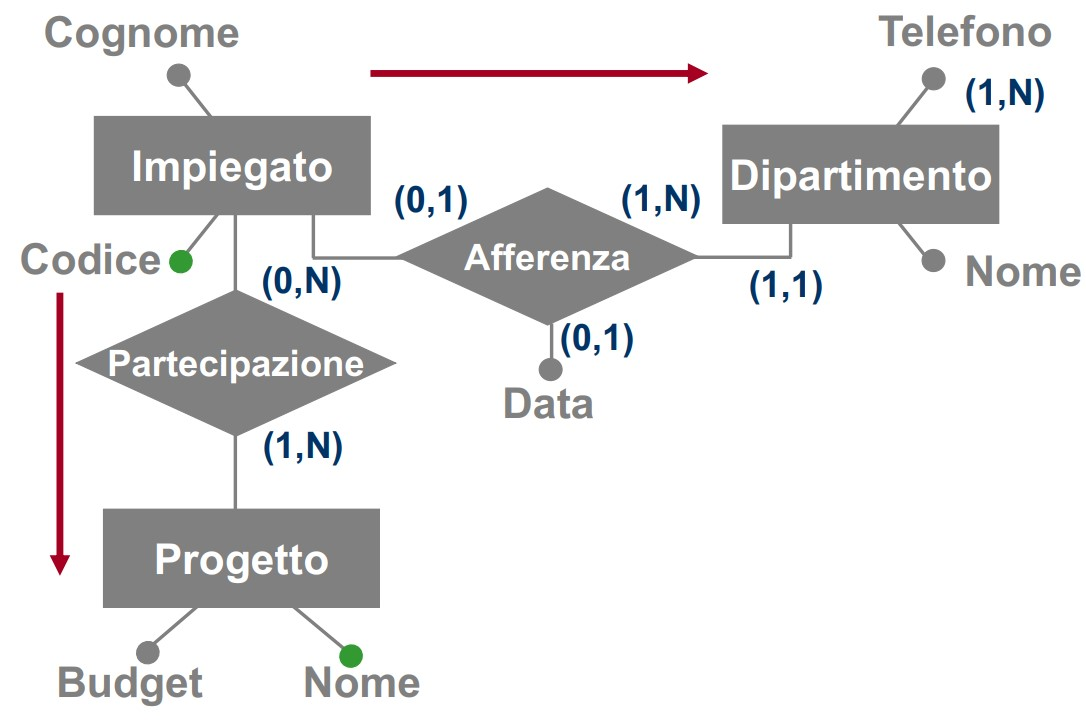
\includegraphics[scale=0.675]{chaptersLezioniSara/img/PLog_tavolaAccessi_es3b.jpg}
\end{center}
Tavola dei volumi:
\begin{center}
    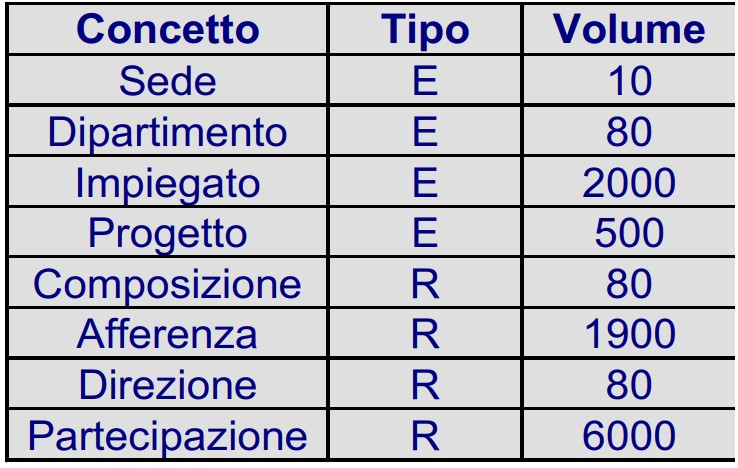
\includegraphics[scale=0.675]{chaptersLezioniSara/img/PLog_tavolaAccessi_es3c.jpg}
\end{center}
Specifica il numero stimato di istanze per ogni entità (E) e associazione (R) dello schema. I valori sono necessariamente approssimati, ma indicativi. Il numero (medio) di partecipazioni di una istanza di entità alle istanze di relazione (dipende dalla cardinalità delle relazioni).

\subsection{Attività della ristrutturazione}
Analisi delle ridondanze.\\
Eliminazione delle generalizzazioni/gerarchie.\\
Partizionamento/accorpamento di entità e relationship.\\
Eliminazione attributi multivalore.\\
Scelta degli identificatori primari

\subsection{Analisi delle ridondanze}
Una ridondanza in uno schema E-R è una informazione significativa ma derivabile da altre.\\
In questa fase si decide se eliminare le ridondanze eventualmente presenti o mantenerle.

\subsection{Ridondanze}
Vantaggi
\begin{itemize}
    \item semplificazione delle interrogazioni
\end{itemize}
Svantaggi
\begin{itemize}
    \item appesantimento degli aggiornamenti
    \item maggiore occupazione di spazio
\end{itemize}

\subsection{Forme di ridondanza in uno schema E-R}
Attributi derivabili:
\begin{itemize}
    \item da altri attributi della stessa entità (o relazione)
    \item da attributi di altre entità (o relazioni)
\end{itemize}
Associazioni derivabili dalla composizione di altre relazioni in presenza di cicli.

\subsubsection{Attributi derivabili}
Il valore di un attributo si calcola sulla base delle altre proprietà.
\begin{center}
    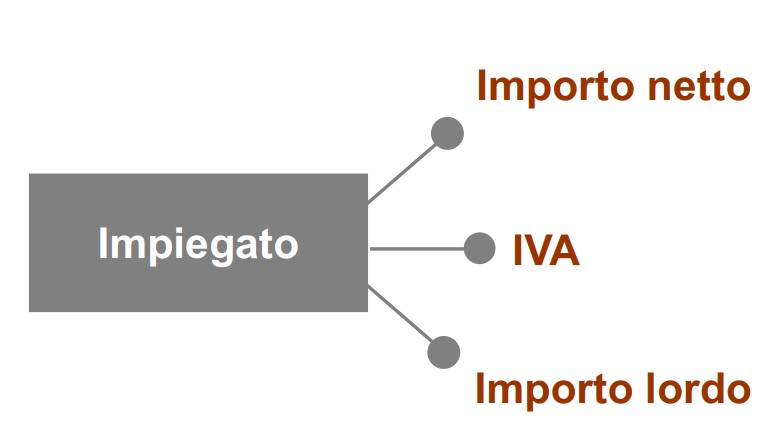
\includegraphics[scale=0.675]{chaptersLezioniSara/img/PLog_ridondanze1.jpg}
\end{center}

\subsubsection{Attributi derivabili da un'altra entità}
Attributo calcolato sulla base degli attributi di un'altra entità.
\begin{center}
    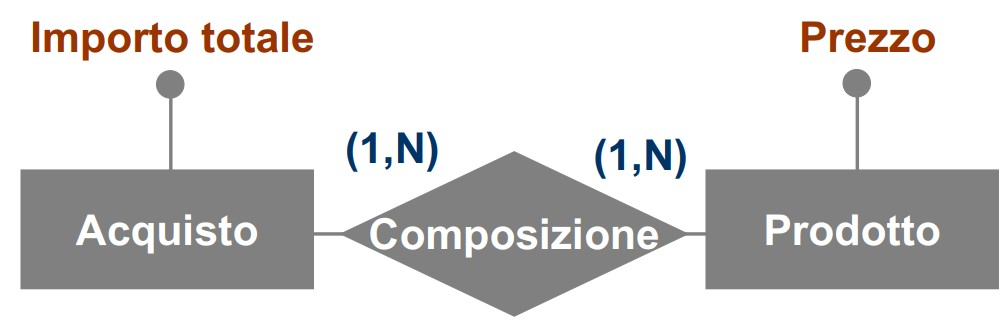
\includegraphics[scale=0.675]{chaptersLezioniSara/img/PLog_ridondanze2.jpg}
\end{center}
\begin{center}
    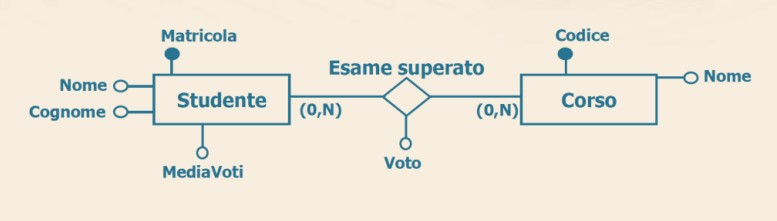
\includegraphics[scale=0.675]{chaptersLezioniSara/img/PLog_ridondanze3.jpg}
\end{center}
L'attributo MediaVoti è ridondante.\\
• utile per velocizzare le interrogazioni relative al calcolo della media dei voti degli studenti.\\
• se conservato, occorre integrare lo schema relazionale con l'indicazione di ridondanza dell'attributo.\\

Vabbeh facciamo che ascolto e basta, mi sono persa.\\
\`E arrivato alla slide 49/142.






